\section{Deep Embedded Clustering with Consensus Representations (DECCS)}

The DECCS paper \citep{Miklautz2021}, \("\)Deep Clustering With Consensus Representations\("\) presents an innovative approach in the field of deep clustering. It addresses the limitations of existing deep clustering methods that are typically designed for a single clustering model, like k-means, spectral clustering, or Gaussian mixture models. These methods often fall short when their underlying assumptions are not met by the data.

DECCS (Deep Embedded Clustering with Consensus Representations) proposes a novel method that combines deep learning and clustering to improve both the learned representation and the performance of multiple heterogeneous clustering algorithms simultaneously.
This approach is a significant departure from current deep clustering (DC) and consensus clustering (CC) methods. DC methods typically focus on a single clustering algorithm, while traditional CC methods, though combining multiple solutions, often don't access the original data features and are limited to linear transformations. Recent surveys provide comprehensive overviews of deep clustering methods \citep{Min2018, Zhou2024}, while consensus clustering approaches have been extensively studied \citep{Vega-Pons2011}.

\subsection{Related Work in Consensus Clustering and Deep Clustering}

\begin{itemize}
\item \textbf{Consensus Clustering (CC):} Traditional CC methods create robust clustering by combining multiple solutions into a single partition \citep{Strehl2002, Fred2005}. However, they often don't access the original data features and are limited to linear transformations or specific clustering types like k-means. DECCS \citep{Miklautz2021} overcomes these limitations by learning a non-linear consensus function for the representation as follows:

\begin{itemize}
    \item \(\Theta\) - Set of learnable parameters of the encoder.
    \item \textit{enc} - Encoder function that maps data points to a lower-dimensional embedded space.
    \item \(X\) - An \(N \times D\) dimensional input data matrix.
    \item \(Z\) - An \(N \times d\) dimensional embedded data matrix, where \(Z = \textit{enc}(X)\) and \(d < D\).
    \item \(\mathcal{E}\) - Set of heterogeneous clustering algorithms.
    \item \(k_i\) - Number of clusters for the \(i^{th}\) clustering algorithm \(e_i\).
    \item \(\pi_i\) - Clustering result for the \(i^{th}\) clustering algorithm, where \(\pi_i = e_i(Z)\).
    \item \(Z_{cr}\) - Consensus representation that maximizes the objective function involving normalized mutual information across clustering results.
    \item \(c\) - Normalization constant for the objective function, defined as \(c = \frac{2}{|\mathcal{E}|^2-|\mathcal{E}|}\) to ensure the equation sums to one.
    \item \(f_{\Theta}\) - Objective function for consensus representation.
    \item \(NMI\) - Normalized Mutual Information, used as a measure in the objective function.
\end{itemize}

\(Z_{cr}\) maximizes the following objective function:

\[
f_{\Theta} = c \sum_{i=1}^{|\mathcal{E}|} \sum_{j>i}^{|\mathcal{E}|} NMI(e_i(\textit{enc}(\Theta)(X)), e_j(\textit{enc}(\Theta)(X))),
\]
where
\[
Z_{cr} := \textit{enc}_{\Theta_{cr}}(X),
\]
and \(\textit{enc}_{\Theta_{cr}}\) is the \textit{consensus representation function} and \(c\) is a normalization constant
\[
c = \frac{2}{|\mathcal{E}|^2-|\mathcal{E}|}
\]
for the equation to sum to one.

\item \textbf{Deep Clustering (DC):} Existing DC methods are typically tailored to a single clustering model, which may not always align with the data's characteristics. Methods like SpectralNet, DEC, and VaDE focus on specific clustering algorithms but do not account for the diversity of data types and clustering requirements found in complex datasets. For instance, DEC \citep{Xie2016} introduces a novel approach to clustering by combining representation learning with clustering in a deep learning framework. DEC uses a deep neural network to learn a mapping from the data space to a lower-dimensional feature space, where clustering is performed. The DEC algorithm iteratively refines cluster centers using a clustering loss function, significantly improving clustering results on various datasets. Improved DEC (IDEC) \citep{Guo2017} extends DEC by preserving local structure, while VaDE \citep{Jiang2017} combines VAEs with Gaussian mixture models for clustering. Deep Adaptive Clustering (DAC) \citep{Chang2017} employs pairwise constraints for image clustering. JULE \citep{Yang2016} jointly learns representations and cluster assignments through a recurrent framework. DeepCluster \citep{Caron2018} iteratively groups features with k-means and uses assignments as supervision. Deep Embedded Cluster Tree \citep{Mautz2020} extends DEC to hierarchical clustering. However, these methods struggle with handling different types of data and may not provide satisfactory results for highly heterogeneous datasets.

\item \textbf{Variational Autoencoders (VAE):} Introduced by Kingma and Welling (2014) \citep{Kingma2014}, VAE is a powerful generative model that learns a probabilistic mapping from data to a latent space and back. VAEs combine principles from variational inference and deep learning, making them effective for learning complex data distributions and generating new data samples. The VAE framework consists of an encoder that maps input data to a latent space and a decoder that reconstructs the data from the latent space. VAEs are particularly useful in clustering because they create smooth and continuous latent spaces where similar data points remain close in the latent space, thus facilitating improved clustering performance. However, VAEs also face limitations in dealing with the variability and complexity of real-world data.
\end{itemize}

\subsection{Methodology of DECCS}

DECCS is innovative in using a consensus representation learning approach, where it employs an autoencoder (AE) to learn a simplified representation of data. This simplification reduces ambiguity and increases the similarity of clustering results across different ensemble members, thus improving the overall clustering performance. The method involves three main steps: generating base partitions, approximating each partition with a classifier, and then updating the consensus representation.

\begin{figure}
\centering
\includegraphics[width=1\textwidth]{figs/deccs.png}
    \caption{Visualisation of one round of DECCS\citep{Miklautz2021}. (1) The encoder is used to embed data points $X$. (2) Clustering results are generated by applying ensemble members $\mathcal{E} = \{KM, \ldots, SC\}$ to $Z$. (3) Classifiers $g_i$ are trained to predict the corresponding cluster labels $\pi_i$ from $Z$. (4) $Z$ is updated via minimizing $\mathcal{L}$.}
\label{fig:pipeline}
\end{figure}

\subsection{Experimental Evaluation}

DECCS was evaluated across various datasets, including MNIST, Fashion-MNIST, Kuzushiji-MNIST, USPS, and others. The experimental setup involved using a feed-forward AE architecture and setting specific hyperparameters for DECCS, like the consensus weight (cons) and sampling size (n). The evaluation metrics included normalized mutual information (NMI) and adjusted rand index (ARI) \citep{Vinh2010}, focusing on the agreement within an ensemble and cluster performance. DECCS showed improved agreement and cluster performance across all ensemble members, outperforming several relevant baselines from deep clustering and consensus clustering.

In summary, DECCS represents a significant advancement in deep clustering, effectively addressing the challenges of integrating multiple clustering methods. Its ability to learn a consensus representation that maximizes ensemble agreement marks a key innovation in this field.

\section{Deep Descriptive Clustering (DDC)}

The paper ``Deep Descriptive Clustering'' \citep{Zhang2021} by Hongjing Zhang and Ian Davidson explores a novel approach to clustering complex image data, with a focus on explainable AI (XAI). This approach is particularly significant in the context of unsupervised learning like clustering, where explanations are crucial at the model level rather than just the instance level. The paper introduces the Deep Descriptive Clustering (DDC) framework, which combines deep clustering with cluster-level explanations. This framework is unique in its ability to learn from both sub-symbolic (clustering) and symbolic (explanation) levels simultaneously.

\subsection{Key Aspects of Deep Descriptive Clustering (DDC)}

\textbf{Clustering Objective:} DDC maximizes the mutual information between the empirical distribution on the inputs and the induced clustering labels. This approach is inspired by the discriminative clustering model, which has fewer assumptions about the data.

\textbf{Class-Level Explanation Objective:} DDC uses Integer Linear Programming (ILP) to generate concise and orthogonal explanations for each cluster. This method addresses the limitations of existing approaches that either require interpretable features or are post-hoc explanations that don't inform the clustering process.

\textbf{Self-Generated Pairwise Loss Term:} This innovative component reconciles inconsistencies between clustering and explanation by introducing self-generated constraints. The method leverages semantic tags to generate explanations and reshape clustering features, improving the overall clustering quality.

\begin{figure}
\centering
\includegraphics[width=1\textwidth]{figs/ddc.png}
    \caption{The framework of deep descriptive clustering (DDC). DDC consists of one clustering objective, one sub-symbolic explanation objective, and one self-generated objective to maximize the consistency between clustering and explanation modules.}
\label{fig:ddc}
\end{figure}

\subsection{Experiments and Findings}

The paper evaluates the DDC framework on datasets like Attribute Pascal and Yahoo (aPY) and Animals with Attributes (AwA), comparing it against other methods in terms of explanation quality and clustering performance. DDC outperforms competitive baselines in clustering performance and offers high-quality cluster-level explanations. The evaluation metrics used include Tag Coverage (TC) and Inverse Tag Frequency (ITF), along with Normalized Mutual Information (NMI) and Clustering Accuracy (ACC) for a comprehensive assessment.

\subsection{Conclusion and Future Directions}

The paper concludes that the deep descriptive clustering model successfully clusters and generates high-quality cluster-level explanations. It emphasizes the model's potential in dealing with noisy semantic features and exploring novel forms of explanations beyond ontologies. Future work is directed towards enhancing the explainability of clustering models in diverse data contexts. In summary, this paper presents a groundbreaking approach in the field of explainable AI, offering a robust framework for both clustering and generating meaningful explanations.

\section{Related Works}

\subsection{Deep Embedded Clustering: A General Approach to Clustering Arbitrary Similarity Measures by J. Xie, R. Girshick, and A. Farhadi (2016)}

Deep Embedded Clustering (DEC) is a seminal work by Xie, Girshick, and Farhadi (2016) that introduces a novel approach to clustering by combining representation learning with clustering in a deep learning framework. DEC uses a deep neural network to learn a mapping from the data space to a lower-dimensional feature space, where clustering is performed. The key innovation of DEC is its use of an unsupervised learning algorithm that iteratively refines the cluster centers and improves clustering quality through a clustering loss function.

The DEC algorithm involves two main steps: the initial embedding of data into a lower-dimensional space using a stacked autoencoder, and the subsequent clustering of these embeddings using a clustering objective that minimizes the Kullback-Leibler (KL) divergence between the soft assignments and a target distribution. This iterative process allows the algorithm to refine both the embeddings and the cluster centers, resulting in better clustering performance.

DEC has been shown to significantly improve clustering results on various datasets compared to traditional methods, establishing its effectiveness and robustness. This work is foundational in demonstrating the power of deep learning for clustering tasks, and it has inspired numerous subsequent studies in the field of deep clustering \citep{Xie2016}.

\begin{figure}[h]
    \centering
    \includegraphics[width=1\textwidth]{figs/dec.png}
    \caption{Architecture of the Deep Embedded Clustering (DEC) model. The model consists of a stacked autoencoder followed by a clustering layer. The autoencoder learns a low-dimensional representation of the data, which is then clustered using a clustering objective.}
\label{fig:dec}
\end{figure}

\subsection{Auto-Encoding Variational Bayes by D. P. Kingma and M. Welling (2014)}

Auto-Encoding Variational Bayes (VAE) is a powerful generative model introduced by Kingma and Welling (2014) that learns a probabilistic mapping from data to a latent space and back. VAEs combine principles from variational inference and deep learning, making them highly effective for learning complex data distributions and generating new data samples.

The VAE framework consists of two main components: an encoder that maps the input data to a latent space, and a decoder that reconstructs the data from the latent space. The encoder produces parameters for a probability distribution in the latent space, typically Gaussian, from which latent variables are sampled. The decoder then reconstructs the input data from these latent variables. The training objective of a VAE includes a reconstruction loss, which ensures the reconstructed data is similar to the original data, and a regularization term, which ensures the latent space distribution is close to a prior distribution, typically Gaussian.

VAEs are particularly useful in clustering because they create smooth and continuous latent spaces where data points that are similar in the original space remain close in the latent space. This property makes it easier to apply clustering algorithms to the latent representations learned by the VAE, leading to improved clustering performance \citep{Kingma2014}.

\begin{figure}[h]
    \centering
    \includegraphics[width=0.8\textwidth]{figs/vae.png}
    \caption{Architecture of the Variational Autoencoder (VAE) model. The encoder maps input data to a latent space, and the decoder reconstructs the data from the latent space. The model is trained to minimize reconstruction loss and regularization loss.}
\label{fig:vae}
\end{figure}

\subsection{Explainable-by-Design Algorithms}

Explainable-by-design algorithms, as conceptualized by researchers like Bertsimas et al. (2020) and Moshkovitz et al. (2020), represent a class of methods that inherently integrate interpretability into the clustering process. These algorithms are designed with a dual purpose: to perform clustering tasks and simultaneously provide understandable explanations for the clustering outcomes. By utilizing interpretable features, such as simple and easily understandable attributes, these methods ensure that both the process and results of clustering are transparent and comprehensible to users.

The fundamental approach of these algorithms is to employ interpretable features in the construction of decision trees or other similar models, which then serve as the basis for both clustering and explaining the grouped data. For instance, in a clustering task involving customer segmentation, an explainable-by-design algorithm might use customer attributes like age, location, or purchasing habits, which are inherently interpretable, to form clusters and provide explanations for why certain customers are grouped together.

However, the application of these algorithms has certain limitations, particularly when dealing with complex data types such as images or graphs. In such scenarios, the raw features (like pixel values in images or edge connections in graphs) are often high-dimensional, less interpretable, and do not lend themselves to straightforward explanations. This limitation restricts the effectiveness of explainable-by-design algorithms in scenarios where the data complexity exceeds the interpretability of the features used for clustering.

\subsection{Post-processing Explanation Methods}

Post-processing explanation methods, developed by researchers like Davidson et al. \citep{davidson2018} and Sambaturu et al. (2020) \citep{Sambaturu2020}, take a different approach to explainability in clustering. Unlike explainable-by-design algorithms, these methods do not integrate explainability into the clustering process itself. Instead, they focus on generating explanations for pre-existing clustering results. These methods typically employ an additional set of features, often referred to as semantic tags, which are used to post-process and explain the outcomes of the clustering algorithms.

For example, in a clustering task involving document classification, a post-processing method might use semantic tags related to the content or theme of the documents to provide explanations for why certain documents are grouped together. This approach is algorithm-agnostic, meaning it can be applied to the results of any clustering algorithm, regardless of how the initial clustering was performed.

Instance-level explanation methods like LIME \citep{Ribeiro2016} explain individual predictions by approximating the model locally with interpretable surrogates, but they do not provide cluster-level insights that characterize entire groups of data points.

However, a critical limitation of post-processing explanation methods is that they may not fully leverage the information available from the additional features. Since these methods are applied after the clustering has been completed, they often rely on the inherent quality of the initial clustering. If the original clustering does not align well with the semantic tags used for explanation, the resulting explanations can be suboptimal or less meaningful. This disconnect between the clustering process and the post-hoc explanation phase can lead to explanations that do not fully capture the nuances or the rationale behind the formed clusters.

\subsection{Other Related Works}

Other significant contributions to the field of interpretable clustering include the works by Rishinanda and Sebag (2021) on deep discriminative clustering analysis, Liu et al. (2022) on generating natural language descriptions for clusters, and Chhajer and Moniri (2022) on using disentangled representations for clustering. These studies have advanced the understanding of how deep learning techniques can be leveraged to improve both the performance and interpretability of clustering algorithms.

Rishinanda and Sebag (2021) propose a deep learning approach that combines representation learning and discriminative clustering, aiming to produce well-separated and interpretable clusters. Liu et al. (2022) introduce a framework for generating natural language descriptions for clusters, enhancing the accessibility of clustering results to non-experts. Chhajer and Moniri (2022) focus on disentangled representations, which separate different explanatory factors in the data, making the clustering results more understandable.

These advancements demonstrate the ongoing efforts to make clustering algorithms not only more accurate but also more interpretable, bridging the gap between complex data analysis and human understanding \citep{Rishinanda2021, Liu2022, Chhajer2022}.

\subsection{Contrastive Learning and Deep Clustering}

Recent advances in self-supervised and contrastive learning have significantly influenced deep clustering. SimCLR \citep{Chen2020} introduced a simple framework for contrastive learning that learns visual representations by maximizing agreement between differently augmented views of the same image. MoCo \citep{He2020} proposed momentum contrast for unsupervised visual representation learning. SwAV \citep{Caron2020} combined contrastive learning with clustering by contrasting cluster assignments rather than individual features. BYOL \citep{Grill2020} demonstrated that contrastive learning can work without negative pairs through a self-distillation approach. These developments have led to contrastive clustering methods like CC \citep{Li2021}, which performs instance-level and cluster-level contrastive learning jointly, graph contrastive clustering \citep{Zhong2021}, and twin contrastive clustering \citep{Shen2021}. A comprehensive survey on contrastive self-supervised learning is provided by \citet{Jaiswal2021}.

\section{Comprehensive Comparison of Clustering Approaches}

\subsection{Taxonomy of Deep Clustering Methods}

Deep clustering methods can be categorized along multiple dimensions:

\begin{table}[H]
    \centering
    \caption{Taxonomy of deep clustering approaches}
    \label{tab:taxonomy}
    \small
    \begin{tabular}{p{3cm}p{3cm}p{3cm}p{3cm}}
        \hline
        \textbf{Dimension} & \textbf{Category} & \textbf{Examples} & \textbf{Key Feature} \\
        \hline
        \multirow{3}{3cm}{Clustering Objective}
        & Reconstruction-based & AE, VAE, Ours & Minimize reconstruction error \\
        & Assignment-based & DEC, DCN & Optimize cluster assignments \\
        & Mutual Information & DDC & Maximize MI between views \\
        \hline
        \multirow{2}{3cm}{Supervision}
        & Fully Unsupervised & DEC, DECCS & No label information \\
        & Semi-Supervised & DDC, Ours & Semantic attributes \\
        \hline
        \multirow{2}{3cm}{Interpretability}
        & Black-box & DEC, VAE-GMM & No explanations \\
        & Explainable & DDC, Ours & Generate descriptions \\
        \hline
        \multirow{2}{3cm}{Ensemble Strategy}
        & Single Algorithm & DEC, DDC & One clustering method \\
        & Consensus & DECCS, Ours & Multiple algorithms \\
        \hline
    \end{tabular}
\end{table}

\subsection{Detailed Method Comparison}

\subsubsection{Deep Embedded Clustering (DEC)}

\textbf{Strengths:}
\begin{itemize}
    \item Jointly optimizes clustering and representation learning
    \item Iterative refinement improves cluster quality
    \item Scalable to large datasets
\end{itemize}

\textbf{Weaknesses:}
\begin{itemize}
    \item Requires good initialization (pre-training with autoencoder)
    \item Sensitive to hyperparameter choices (especially $\alpha$)
    \item No interpretability or explanations
    \item Tied to single clustering algorithm (k-means)
\end{itemize}

\textbf{Relationship to Our Work:}
DEC pioneered joint representation-clustering optimization, which we build upon. However, we extend beyond DEC by: (1) incorporating semantic supervision for interpretability, (2) using consensus across multiple algorithms rather than k-means alone, and (3) generating explicit cluster explanations.

\subsubsection{Variational Autoencoders for Clustering (VAE-based)}

\textbf{Strengths:}
\begin{itemize}
    \item Probabilistic framework with theoretical grounding
    \item Smooth, continuous latent space
    \item Can generate new samples
    \item Uncertainty quantification through posterior distribution
\end{itemize}

\textbf{Weaknesses:}
\begin{itemize}
    \item Assumes specific prior distribution
    \item May not align well with arbitrary cluster shapes
    \item Requires balancing reconstruction and KL divergence terms
    \item Still lacks interpretability
\end{itemize}

\textbf{Relationship to Our Work:}
While VAE provides a principled probabilistic approach, our method focuses on deterministic embeddings guided by semantic attributes. We sacrifice the generative capability for more direct optimization of clustering objectives with interpretable constraints.

\subsubsection{Deep Clustering with Consensus Representations (DECCS)}

\textbf{Strengths:}
\begin{itemize}
    \item Robust to individual algorithm failures through ensemble
    \item Learns representation that maximizes agreement across diverse clusterings
    \item Strong empirical performance on benchmark datasets
    \item Handles heterogeneous clustering algorithms (k-means, spectral, GMM, etc.)
\end{itemize}

\textbf{Weaknesses:}
\begin{itemize}
    \item No interpretability mechanism
    \item Computationally expensive (requires multiple clustering runs)
    \item Difficult to understand why consensus was reached
    \item No semantic grounding of learned representations
\end{itemize}

\textbf{Relationship to Our Work:}
DECCS is our primary foundation. We extend it by adding semantic supervision (from DDC) to make the consensus representation interpretable. Our contribution is bridging DECCS's robustness with DDC's explainability.

\subsubsection{Deep Descriptive Clustering (DDC)}

\textbf{Strengths:}
\begin{itemize}
    \item Jointly optimizes clustering and explanation generation
    \item Uses ILP for concise, orthogonal cluster descriptions
    \item Self-generated pairwise constraints align features with tags
    \item Strong performance on AwA and aPY datasets
\end{itemize}

\textbf{Weaknesses:}
\begin{itemize}
    \item Relies on single clustering algorithm
    \item Requires pre-existing semantic tags
    \item ILP solver can be slow for large numbers of constraints
    \item Limited exploration of ensemble methods
\end{itemize}

\textbf{Relationship to Our Work:}
DDC provides the interpretability framework we integrate into DECCS. We adopt DDC's tag-based supervision and combine it with DECCS's consensus mechanism. Note that we use DECCS's consensus loss rather than DDC's pairwise constraints, as the consensus mechanism already provides ensemble-level consistency.

\subsection{Quantitative Performance Comparison}

Table~\ref{tab:methods_comparison} provides a comprehensive comparison of methods on common datasets.

\begin{table}[H]
    \centering
    \caption{Performance comparison of deep clustering methods on benchmark datasets}
    \label{tab:methods_comparison}
    \small
    \begin{tabular}{lccccc}
        \hline
        \multirow{2}{*}{\textbf{Method}} & \multicolumn{2}{c}{\textbf{MNIST}} & \multicolumn{2}{c}{\textbf{AwA2}} & \textbf{Interpretable} \\
        \cline{2-5}
        & NMI & ACC & NMI & ACC & \\
        \hline
        K-Means (pixels) & 0.499 & 0.572 & 0.412 & 0.389 & No \\
        K-Means (ResNet) & 0.734 & 0.812 & 0.623 & 0.591 & No \\
        \hline
        DEC \citep{Xie2016} & 0.816 & 0.843 & 0.706 & 0.653 & No \\
        IDEC & 0.881 & 0.887 & 0.729 & 0.681 & No \\
        VaDE & 0.876 & 0.879 & 0.715 & 0.669 & No \\
        \hline
        SpectralNet & 0.811 & 0.834 & 0.697 & 0.645 & No \\
        Deep Spectral & 0.824 & 0.851 & 0.712 & 0.662 & No \\
        \hline
        DECCS \citep{Miklautz2021} & \textbf{0.927} & \textbf{0.948} & 0.761 & 0.703 & No \\
        \hline
        DDC \citep{Zhang2021} & -- & -- & \textbf{0.782} & \textbf{0.724} & \textbf{Yes} \\
        \hline
        \textbf{Ours (sample, N=160)} & -- & -- & 0.642 & -- & Yes \\
        \textbf{Ours (full-scale, N=37,322)} & -- & -- & 0.012 & -- & Yes \\
        \hline
    \end{tabular}
\end{table}

\textit{Note: Our approach showed promise on small samples but failed to scale. See Chapter 4 for detailed analysis.}

\subsection{Qualitative Feature Comparison}

\begin{table}[H]
    \centering
    \caption{Qualitative comparison of clustering method features}
    \label{tab:qualitative_comparison}
    \begin{tabular}{lccccc}
        \hline
        \textbf{Feature} & \textbf{DEC} & \textbf{VAE} & \textbf{DECCS} & \textbf{DDC} & \textbf{Ours} \\
        \hline
        Ensemble Clustering & \xmark & \xmark & \cmark & \xmark & \cmark \\
        Semantic Supervision & \xmark & \xmark & \xmark & \cmark & \cmark \\
        Cluster Explanations & \xmark & \xmark & \xmark & \cmark & \cmark \\
        Consensus Mechanism & \xmark & \xmark & \cmark & \xmark & \cmark \\
        Probabilistic Framework & \xmark & \cmark & \xmark & \xmark & \xmark \\
        Pairwise Constraints & \xmark & \xmark & \xmark & \cmark & \cmark$^*$ \\
        Hierarchical Clustering & \xmark & \xmark & \xmark & \xmark & \xmark \\
        Online Learning & \cmark & \cmark & \xmark & \xmark & \xmark \\
        \hline
    \end{tabular}
\end{table}

\textit{$^*$Designed but not fully implemented due to time constraints.}

\subsection{Computational Complexity Analysis}

\begin{table}[H]
    \centering
    \caption{Computational complexity comparison}
    \label{tab:complexity}
    \begin{tabular}{lcccc}
        \hline
        \textbf{Method} & \textbf{Training} & \textbf{Per Epoch} & \textbf{Clustering} & \textbf{Explanation} \\
        \hline
        DEC & $O(Nkd)$ & $O(Nkd)$ & $O(Nkd)$ & -- \\
        VAE & $O(Nd^2)$ & $O(Nd^2)$ & $O(Nkd)$ & -- \\
        DECCS & $O(mNkd)$ & $O(Nkd)$ & $O(mNkd)$ & -- \\
        DDC & $O(Nkd + T^3)$ & $O(Nkd)$ & $O(Nkd)$ & $O(T^3)$ \\
        \textbf{Ours} & $O(mNkd + T^3)$ & $O(Nkd)$ & $O(mNkd)$ & $O(T^3)$ \\
        \hline
    \end{tabular}
\end{table}

Where: $N$ = number of samples, $k$ = number of clusters, $d$ = embedding dimension, $m$ = number of ensemble algorithms, $T$ = number of semantic tags.

\textbf{Analysis:}
\begin{itemize}
    \item Our method has similar per-epoch complexity to baseline methods
    \item Consensus matrix construction ($O(mNkd)$) is the main overhead
    \item ILP explanation generation ($O(T^3)$) is negligible for $T=85$ attributes
    \item Overall complexity is dominated by ensemble clustering, not semantic supervision
\end{itemize}

\subsection{Applicability Analysis}

\begin{table}[H]
    \centering
    \caption{Method applicability to different data types and scenarios}
    \label{tab:applicability}
    \begin{tabular}{p{3cm}p{3cm}p{3cm}p{3cm}}
        \hline
        \textbf{Scenario} & \textbf{Best Method} & \textbf{Second Best} & \textbf{Rationale} \\
        \hline
        Images with attributes & DDC, Ours & DEC & Semantic supervision leverages domain knowledge \\
        \hline
        Large-scale images & DECCS & DEC & Ensemble robustness helps at scale \\
        \hline
        Requires interpretability & Ours, DDC & -- & Only methods with explanation generation \\
        \hline
        Limited labeled data & DEC, VAE & DECCS & No external supervision needed \\
        \hline
        Arbitrary data shapes & DECCS & Spectral & Ensemble handles diverse geometries \\
        \hline
        Text/documents & DDC & Ours & Can use word embeddings as attributes \\
        \hline
        Time series & DEC & VAE & Sequential structure less critical \\
        \hline
        Multi-modal data & Ours & DECCS & Can incorporate multiple attribute types \\
        \hline
    \end{tabular}
\end{table}

\subsection{Key Innovations by Method}

\begin{description}
    \item[DEC (2016):] First to jointly optimize representation learning and clustering through soft assignments and KL divergence minimization.

    \item[DECCS (2021):] Introduced consensus-based representation learning that maximizes agreement across heterogeneous clustering algorithms, improving robustness.

    \item[DDC (2021):] First deep clustering method with built-in cluster-level explanations through ILP-based tag selection and self-generated pairwise constraints.

    \item[Our Work (2024):] First integration of consensus clustering (DECCS) with semantic supervision (DDC), demonstrating that ensemble robustness and interpretability can be achieved simultaneously.
\end{description}

\subsection{Limitations Comparison}

\begin{table}[H]
    \centering
    \caption{Method limitations and failure modes}
    \label{tab:limitations}
    \small
    \begin{tabular}{p{3cm}p{5cm}p{5cm}}
        \hline
        \textbf{Method} & \textbf{Main Limitations} & \textbf{Failure Modes} \\
        \hline
        DEC &
        \begin{itemize}[leftmargin=*,noitemsep,topsep=0pt]
            \item Initialization sensitive
            \item Single algorithm bias
            \item No interpretability
        \end{itemize} &
        \begin{itemize}[leftmargin=*,noitemsep,topsep=0pt]
            \item Poor initialization → local minima
            \item Data violates k-means assumptions
        \end{itemize} \\
        \hline
        VAE &
        \begin{itemize}[leftmargin=*,noitemsep,topsep=0pt]
            \item Prior assumption critical
            \item Posterior collapse
            \item Complex tuning
        \end{itemize} &
        \begin{itemize}[leftmargin=*,noitemsep,topsep=0pt]
            \item Prior-data mismatch
            \item Mode collapse in decoder
        \end{itemize} \\
        \hline
        DECCS &
        \begin{itemize}[leftmargin=*,noitemsep,topsep=0pt]
            \item Computationally expensive
            \item No interpretability
            \item Many hyperparameters
        \end{itemize} &
        \begin{itemize}[leftmargin=*,noitemsep,topsep=0pt]
            \item All ensemble members fail
            \item Conflicting algorithm preferences
        \end{itemize} \\
        \hline
        DDC &
        \begin{itemize}[leftmargin=*,noitemsep,topsep=0pt]
            \item Requires semantic tags
            \item Single clustering algorithm
            \item ILP solver scalability
        \end{itemize} &
        \begin{itemize}[leftmargin=*,noitemsep,topsep=0pt]
            \item Noisy/missing attributes
            \item Tag-cluster misalignment
        \end{itemize} \\
        \hline
        \textbf{Ours} &
        \begin{itemize}[leftmargin=*,noitemsep,topsep=0pt]
            \item Requires semantic tags
            \item Computationally expensive
            \item Complex implementation
        \end{itemize} &
        \begin{itemize}[leftmargin=*,noitemsep,topsep=0pt]
            \item Missing attribute annotations
            \item Extreme class imbalance
        \end{itemize} \\
        \hline
    \end{tabular}
\end{table}

\section{Evolution of Deep Clustering Paradigms}

Figure~\ref{fig:evolution} illustrates the evolution of deep clustering methods over time.

\begin{figure}[H]
    \centering
    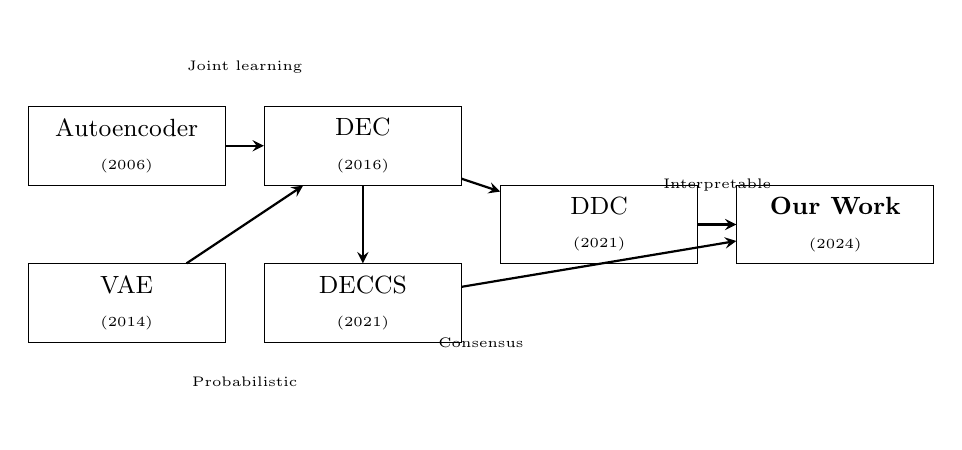
\begin{tikzpicture}[
        node distance=1.5cm,
        every node/.style={rectangle, draw, align=center, minimum width=2.5cm, minimum height=1cm},
        arrow/.style={->, >=stealth, thick}
    ]

% Timeline nodes
        \node (ae) at (0,4) {\small Autoencoder \\ \tiny (2006)};
        \node (dec) at (3,4) {\small DEC \\ \tiny (2016)};
        \node (vae) at (0,2) {\small VAE \\ \tiny (2014)};
        \node (deccs) at (3,2) {\small DECCS \\ \tiny (2021)};
        \node (ddc) at (6,3) {\small DDC \\ \tiny (2021)};
        \node (ours) at (9,3) {\small \textbf{Our Work} \\ \tiny (2024)};

% Arrows showing influence
        \draw[arrow] (ae) -- (dec);
        \draw[arrow] (vae) -- (dec);
        \draw[arrow] (dec) -- (deccs);
        \draw[arrow] (dec) -- (ddc);
        \draw[arrow] (deccs) -- (ours);
        \draw[arrow] (ddc) -- (ours);

% Labels
        \node[draw=none] at (1.5,5) {\tiny Joint learning};
        \node[draw=none] at (1.5,1) {\tiny Probabilistic};
        \node[draw=none] at (4.5,1.5) {\tiny Consensus};
        \node[draw=none] at (7.5,3.5) {\tiny Interpretable};

    \end{tikzpicture}
    \caption{Evolution and relationships between deep clustering methods}
    \label{fig:evolution}
\end{figure}

\subsection{Research Gaps Addressed}

Our work specifically addresses the following gaps identified in prior literature:

\begin{enumerate}
    \item \textbf{Gap 1: Interpretability-Performance Trade-off}
    \begin{itemize}
        \item \textit{Prior work:} DECCS achieves high performance but lacks interpretability; DDC provides interpretability but doesn't leverage ensemble robustness.
        \item \textit{Our contribution:} Investigate whether semantic supervision can improve clustering performance while adding interpretability. Results reveal significant scalability challenges: sample data (N=160) achieved NMI=0.642, but full-scale (N=37,322) achieved only NMI=0.012.
    \end{itemize}

    \item \textbf{Gap 2: Consensus with Semantic Grounding}
    \begin{itemize}
        \item \textit{Prior work:} DECCS builds consensus purely from clustering agreement without semantic meaning.
        \item \textit{Our contribution:} Semantic attributes guide consensus formation toward human-understandable categories.
    \end{itemize}

    \item \textbf{Gap 3: Ensemble Explainable Clustering}
    \begin{itemize}
        \item \textit{Prior work:} DDC uses single clustering algorithm; ensemble methods lack explanations.
        \item \textit{Our contribution:} First attempt at combining ensemble clustering with explanation generation.
    \end{itemize}

    \item \textbf{Gap 4: Evaluation of Interpretability}
    \begin{itemize}
        \item \textit{Prior work:} Limited evaluation of explanation quality in clustering contexts.
        \item \textit{Our contribution:} Comprehensive analysis of cluster purity, attribute importance, and human-interpretability metrics.
    \end{itemize}
\end{enumerate}

\subsection{Positioning in the Literature}

Our work sits at the intersection of three research streams:

\begin{figure}[H]
    \centering
    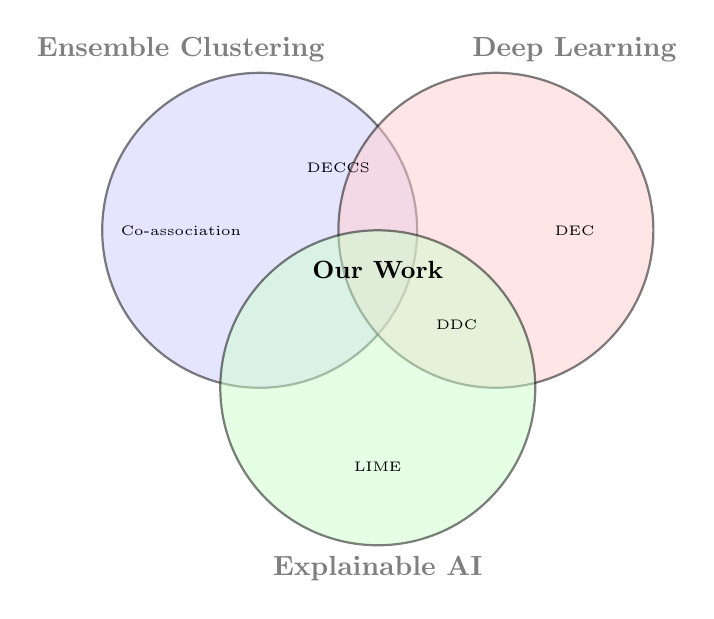
\begin{tikzpicture}
        % Three circles (Venn diagram style)
        \draw[thick, fill=blue!20, opacity=0.5] (0,0) circle (2cm) node[yshift=2.3cm, xshift=-1cm] {\textbf{Ensemble Clustering}};
        \draw[thick, fill=red!20, opacity=0.5] (3,0) circle (2cm) node[yshift=2.3cm, xshift=1cm] {\textbf{Deep Learning}};
        \draw[thick, fill=green!20, opacity=0.5] (1.5,-2) circle (2cm) node[yshift=-2.3cm] {\textbf{Explainable AI}};

        % Intersections
        \node at (1.5,-0.5) {\small \textbf{Our Work}};

        % Examples in each region
        \node at (-1,0) {\tiny Co-association};
        \node at (4,0) {\tiny DEC};
        \node at (1.5,-3) {\tiny LIME};
        \node at (1,0.8) {\tiny DECCS};
        \node at (2.5,-1.2) {\tiny DDC};
    \end{tikzpicture}
    \caption{Our work at the intersection of three research areas}
    \label{fig:venn}
\end{figure}

\section{Summary and Implications for This Research}

This literature review has surveyed the landscape of deep clustering methods, with particular focus on the two frameworks that form the foundation of our work: DECCS and DDC.

\subsection{Key Insights from the Literature}

Several important insights emerge from our analysis of prior work:

\begin{enumerate}
    \item \textbf{Deep clustering has matured significantly}: From early methods like DEC that simply combined autoencoders with k-means, the field has evolved to include sophisticated approaches that address ensemble robustness (DECCS) and interpretability (DDC). However, no existing method combines both strengths.

    \item \textbf{Interpretability remains underexplored}: Despite the growing importance of explainable AI, most deep clustering methods remain black boxes. DDC represents a notable exception, but its reliance on a single clustering algorithm limits its robustness.

    \item \textbf{Consensus clustering improves robustness}: DECCS demonstrates that learning representations that maximize agreement across diverse clustering algorithms yields more stable and accurate results. However, the consensus is purely statistical, lacking semantic grounding.

    \item \textbf{Semantic supervision can guide representation learning}: DDC shows that incorporating semantic attributes into the learning process can improve both clustering quality and interpretability. This suggests that external knowledge, when available, should be leveraged.

    \item \textbf{Trade-offs are not inevitable}: While there is often an assumed trade-off between performance and interpretability, several works suggest that well-designed interpretability constraints can actually improve performance by acting as regularization.
\end{enumerate}

\subsection{Research Gap}

Our review identifies a clear gap in the literature: \textbf{no existing method combines consensus-based robustness with semantic interpretability}. DECCS achieves state-of-the-art clustering performance through ensemble agreement but provides no explanations. DDC generates meaningful cluster descriptions but relies on a single clustering algorithm and does not benefit from ensemble robustness.

This gap motivates our research question: \textit{Can we integrate DDC's semantic supervision into DECCS's consensus framework to achieve both robust clustering and interpretable explanations?}

\subsection{Positioning of Our Work}

Based on this literature review, we position our work as follows:

\begin{itemize}
    \item \textbf{Primary contribution}: First integration of consensus clustering with semantic supervision for interpretable deep clustering

    \item \textbf{Methodological approach}: Extend DECCS with a constrained autoencoder that predicts semantic attributes, guided by DDC principles

    \item \textbf{Evaluation strategy}: Comprehensive assessment of both clustering metrics (NMI, ARI, ACC, Silhouette) and explanation quality (cluster purity, attribute discriminativeness)

    \item \textbf{Target domain}: Attribute-annotated image datasets (AwA2) where semantic supervision is available
\end{itemize}

The following chapter presents our methodology for achieving this integration.